\documentclass{beamer}
\usetheme{Boadilla}
\usepackage{graphicx}
\usepackage[final]{animate}
\usepackage{breqn}
\usepackage{xcolor}
\usepackage{booktabs}
\usepackage{pgf}
\usepackage{caption}

% change format of enumerated lists
\setbeamertemplate{enumerate items}[default]
\setbeamertemplate{navigation symbols}{}

% macros
\newcommand{\emtxt}[1]{\textbf{\textit{{\color{mypal4} #1}}}}

% change font size for figure captions
\setbeamerfont{caption}{size=\scriptsize}

\usefonttheme{serif}

% custom colors
\definecolor{mypal1}{HTML}{FFF7FD}\definecolor{mypal2}{HTML}{D7CEE9}\definecolor{mypal3}{HTML}{76A6D0}\definecolor{mypal4}{HTML}{00828B}\definecolor{mypal5}{HTML}{004533}
% setup

% get online bib file

\setbeamercolor{title}{fg=mypal5} % main title
\setbeamercolor{frametitle}{fg=mypal4, bg=mypal2} % frame titles
\setbeamercolor{structure}{fg=mypal4} % bottom banner
\setbeamercolor{normal text}{fg=mypal5}
\usebackgroundtemplate{
\includegraphics[height=\paperheight,width=\paperwidth]{fig/back_tmp.pdf}}

\usepackage{Sweave}
\begin{document}
\Sconcordance{concordance:Beck_etal_CERF_2019.tex:Beck_etal_CERF_2019.Rnw:%
1 22 1 1 20 1 1 1 13 1 1 1 6 7 1 1 0 242 1}


\title[Tracking SF Bay Water Quality]{Tracking San Francisco Bay water quality using generalized additive models in an R Shiny framework}
\author[Beck et al.]{Marcus W. Beck\inst{1} \and Ian Wren\inst{2} \and Rebecca Murphy\inst{3} \and \\ Perry de Valpine\inst{4} \and David Senn\inst{5}}

\institute[TBEP]{$^1$Tampa Bay Estuary Program\\ $^2$San Francisco Baykeeper \\$^3$Cheseapeake Bay Program \\$^4$University of California Berkeley \\$^5$San Francisco Estuary Institute}

\date{Nov. 4, 2019}

\titlegraphic{
\vspace{-0.1in}
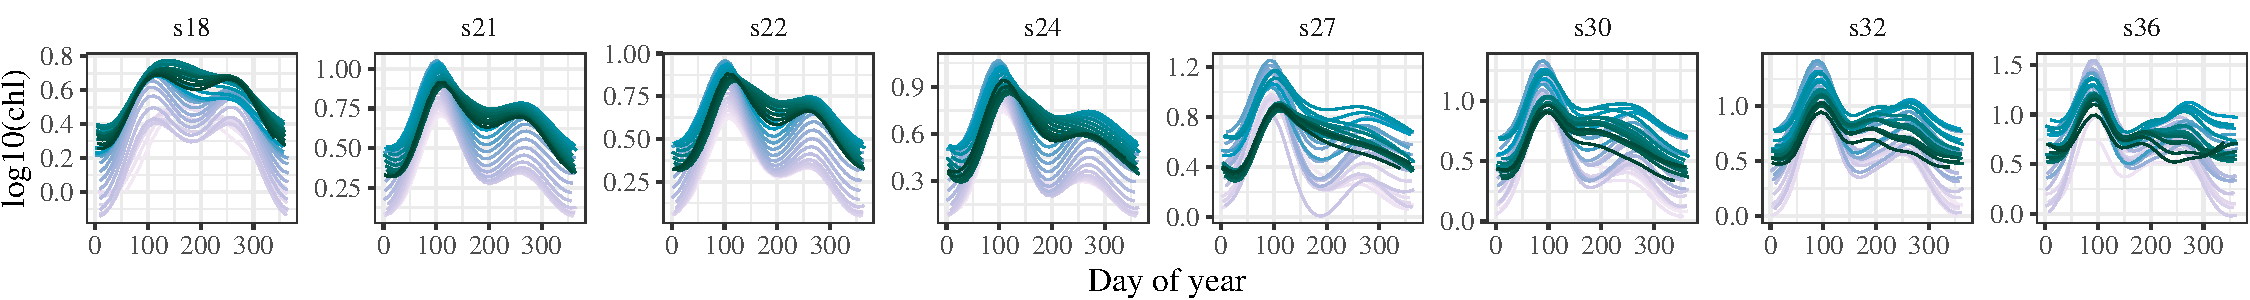
\includegraphics[width=\linewidth]{fig/titlegraph.pdf}
}

%%%%%%
\begin{frame}
% \vspace{0.2in}
\titlepage
\end{frame}

\section{Background}

%%%%%%
\begin{frame}{\textbf{Why do we care about trends?} \hspace{0pt plus 1 filll} $\vcenter{\hbox{
\includegraphics[width=0.15\paperwidth]{fig/logo.png}}}$}
\begin{itemize}
\item Provide information on natural variation of water quality parameters - identify 1st order principles to understand a system  \\~\\
\item Document historical changes in response to management actions - did investments make a difference? \\~\\
\item Anticipate future changes with proposed restoration or management - understand the past to predict the future
\end{itemize}
\end{frame}

%%%%%%
\begin{frame}{\textbf{Trends vary in space and time} \hspace{0pt plus 1 filll} $\vcenter{\hbox{
\includegraphics[width=0.15\paperwidth]{fig/logo.png}}}$}
\centerline{\emtxt{Observed data represent effects from many processes}}
\vspace{0.15in}
\centerline{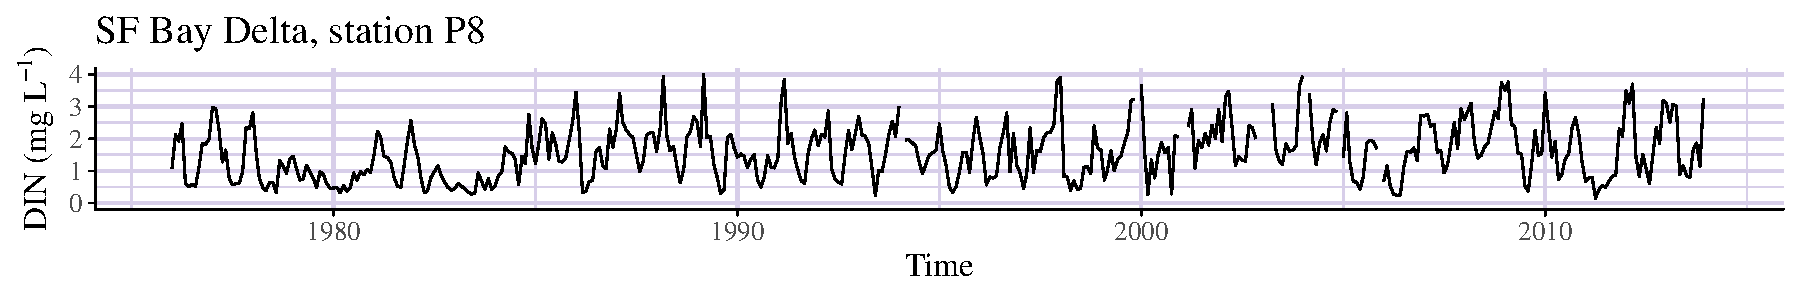
\includegraphics[width = \textwidth]{fig/ts_ex.pdf}}
\vspace{0.15in}
\begin{columns}[t]
\begin{column}{0.3\textwidth}
{\bf \underline{\emtxt{Climate}}}\\
precipitation\\
temperature\\
wind events\\
ENSO effects
\end{column}
\begin{column}{0.3\textwidth}
{\bf \underline{\emtxt{Local}}}\\
light/turbidity\\
residence time\\
invasive species\\
trophic effects
\end{column}
\begin{column}{0.3\textwidth}
{\bf \underline{\emtxt{Regional/historical}}}\\
watershed inputs\\
point sources\\
management actions
flow changes
\end{column}
\end{columns}
\end{frame}

%%%%%%
\begin{frame}{\textbf{Must translate data into information} \hspace{0pt plus 1 filll} $\vcenter{\hbox{
\includegraphics[width=0.15\paperwidth]{fig/logo.png}}}$}
\onslide<+->
\centerline{\emtxt{Observed data represents effects of many processes}}
\vspace{0.15in}
\centerline{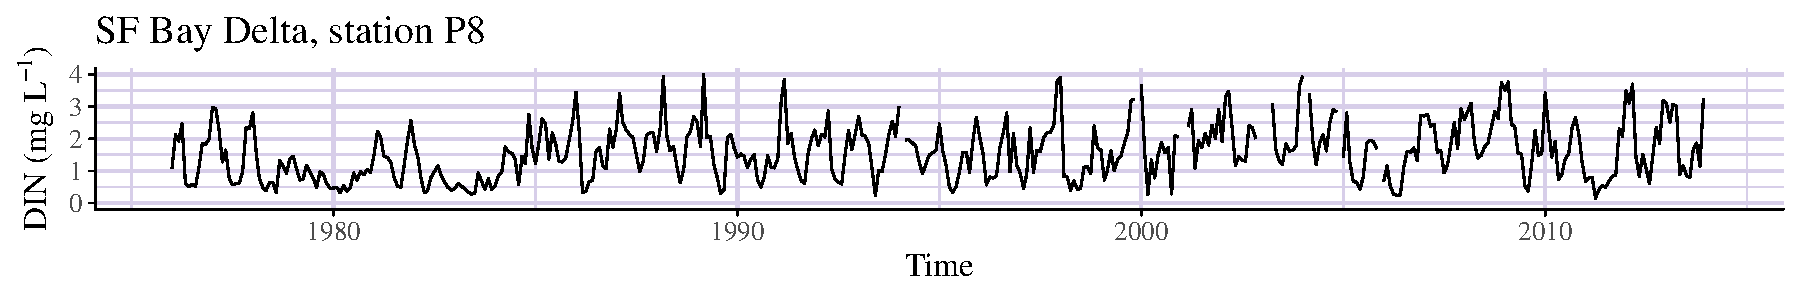
\includegraphics[width = \textwidth]{fig/ts_ex.pdf}}
\centerline{\emtxt{Models should describe components to evaluate effects}}
\vspace{-0.1in}
\begin{columns}[t]
\begin{column}{0.5\textwidth}
\onslide<+->{
\centerline{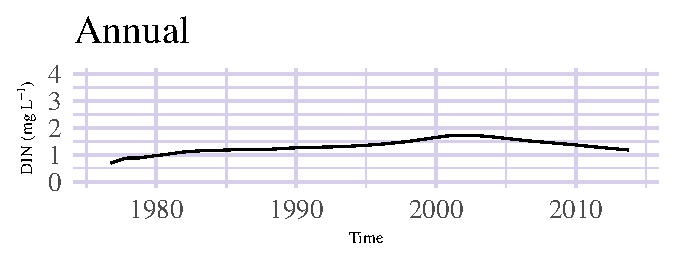
\includegraphics[width = 0.8\textwidth]{fig/schematic2.pdf}}
\centerline{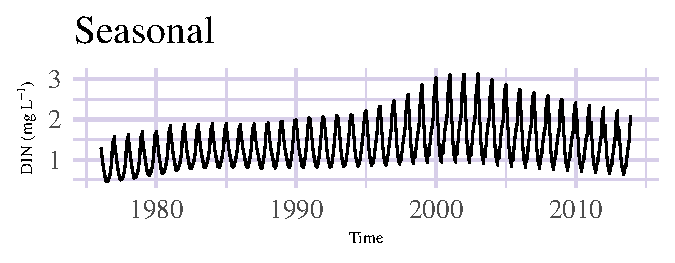
\includegraphics[width = 0.8\textwidth]{fig/schematic3.pdf}}
}
\end{column}
\begin{column}{0.5\textwidth}
\onslide<+->{
\centerline{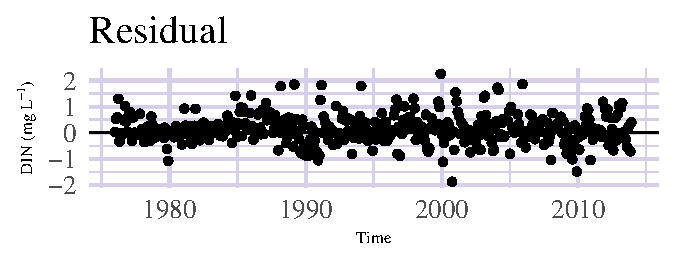
\includegraphics[width = 0.8\textwidth]{fig/schematic4.pdf}}
\centerline{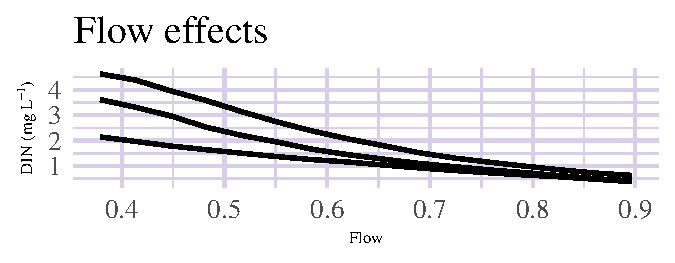
\includegraphics[width = 0.8\textwidth]{fig/schematic5.pdf}}
}
\end{column}
\end{columns}
\end{frame}

\section{Methods}

%%%%%%
\begin{frame}{\textbf{South San Francisco Bay} \hspace{0pt plus 1 filll} $\vcenter{\hbox{
\includegraphics[width=0.15\paperwidth]{fig/logo.png}}}$}
\begin{columns}
\begin{column}{0.5\textwidth}
\begin{itemize}
\onslide<1->
\item Historically a high-nutrients, high-turbidity, low-productivity system {\tiny \cite{Cole84,Alpine88}} \\~\\
\onslide<2->
\item Recent increases observed in summer-fall chl-a concentrations {\tiny \cite{Cloern07,Cloern12b}} \\~\\
\onslide<3->
\item Lead to creation of a Nutrient Management Strategy (NMS) to characterize status/trends and management needs 
\end{itemize}
\end{column}
\begin{column}{0.5\textwidth}
\onslide<1->
\centerline{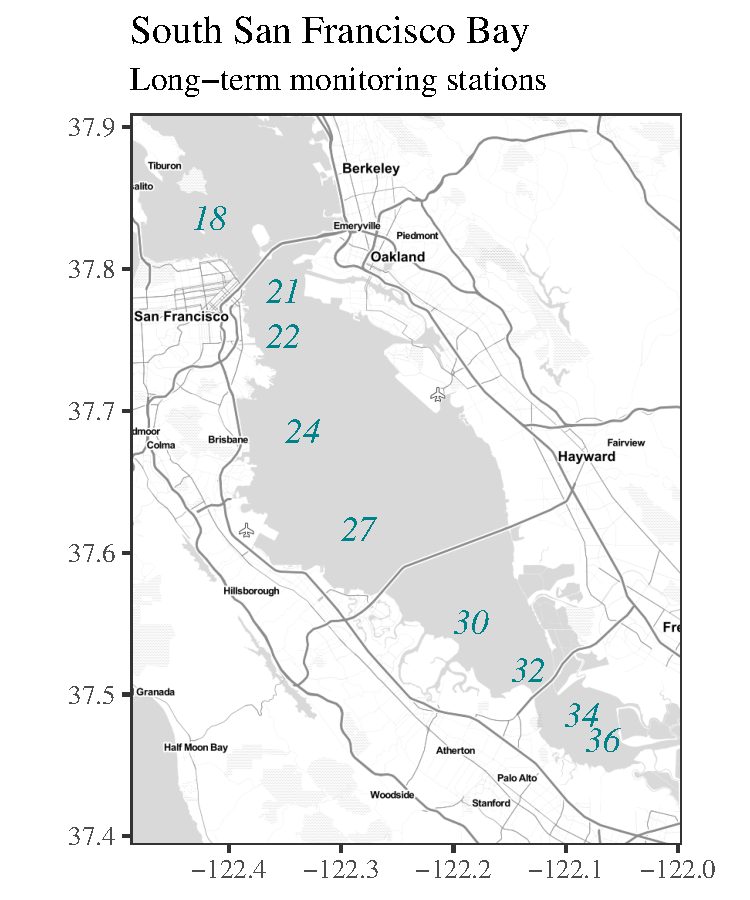
\includegraphics[width = 0.95\textwidth]{fig/map.pdf}}
\end{column}
\end{columns}
\end{frame}

%%%%%%
\begin{frame}{\textbf{South San Francisco Bay} \hspace{0pt plus 1 filll} $\vcenter{\hbox{
\includegraphics[width=0.15\paperwidth]{fig/logo.png}}}$}
\begin{columns}
\begin{column}{0.5\textwidth}
\onslide<1->
Questions of concern: \\~\\
\begin{itemize}
\onslide<2->
\item Since changes are visually apparent, which are significant?  \\~\\
\onslide<3->
\item What has been the estimated rate and direction of any linear or non-monotonic change? \\~\\
\onslide<4->
\item Do any of these changes coincide with changes in other water quality parameters?
\end{itemize}
\end{column}
\begin{column}{0.5\textwidth}
\onslide<1->
\centerline{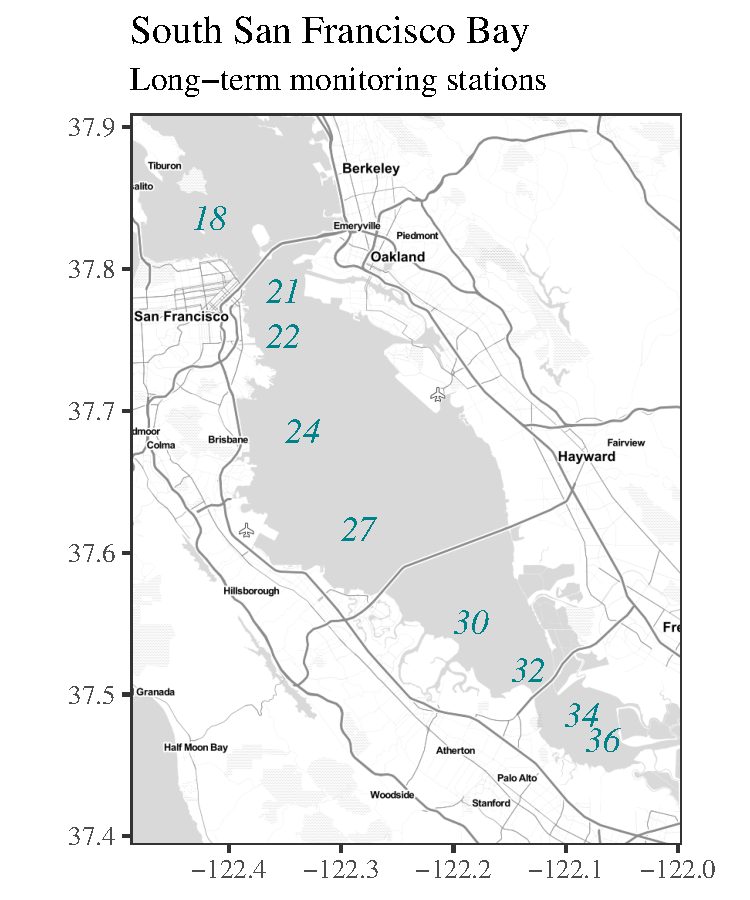
\includegraphics[width = 0.95\textwidth]{fig/map.pdf}}
\end{column}
\end{columns}
\end{frame}

%%%%%%
\begin{frame}{\textbf{Application of additive models} \hspace{0pt plus 1 filll} $\vcenter{\hbox{
\includegraphics[width=0.15\paperwidth]{fig/logo.png}}}$}
\begin{itemize}
\item The Chesapeake Bay Program (CBP) has been wrestling with similar issues, i.e., can a flexible statistical analysis method be applied to evaluate significant, non-linear changes in water quality parameters? {\tiny \cite{Beck17,Murphy19}} \\~\\
\item We applied Generalized Additive Models (GAMs) developed by CBP to characterize long-term trends at nine stations over thirty years in South SF Bay \\~\\
\item An interactive website was also developed using R Shiny to explore trends and communicate results with stakeholders
\end{itemize}
\end{frame}

%%%%%%
\begin{frame}{\textbf{Application of additive models} \hspace{0pt plus 1 filll} $\vcenter{\hbox{
\includegraphics[width=0.15\paperwidth]{fig/logo.png}}}$}
For each station, chlorophyll was modelled as a function of annual and seasonal changes over time {\tiny baytrends R package, \cite{Murphy19b}}\\~\\
Four GAMs were evaluated and compared using standard methods for model comparison (AIC, R\textsuperscript{2}, GCV) \\~\\
\begin{itemize}
\item \texttt{gam0}: chl $\sim$ year + s(doy)
\item \texttt{gam1}: chl $\sim$ year + s(doy) + s(year)
\item \texttt{gam2}: chl $\sim$ year + s(doy) + s(year) + ti(doy, year)
\item \texttt{gam6}: chl $\sim$ year + s(doy) + s(year, k = large)
\end{itemize}
\end{frame}

%%%%%%
\begin{frame}{\textbf{Application of additive models} \hspace{0pt plus 1 filll} $\vcenter{\hbox{
\includegraphics[width=0.15\paperwidth]{fig/logo.png}}}$}
\only<1>{\texttt{gam0}: chl $\sim$ year + s(doy)}
\only<2>{\texttt{gam1}: chl $\sim$ year + s(doy) + s(year)}
\only<3>{\texttt{gam2}: chl $\sim$ year + s(doy) + s(year) + ti(doy, year)}
\only<4>{\texttt{gam6}: chl $\sim$ year + s(doy) + s(year, k = large)}
\begin{columns}
\begin{column}{0.5\textwidth}
\begin{figure}
\begin{overprint}
\onslide<1>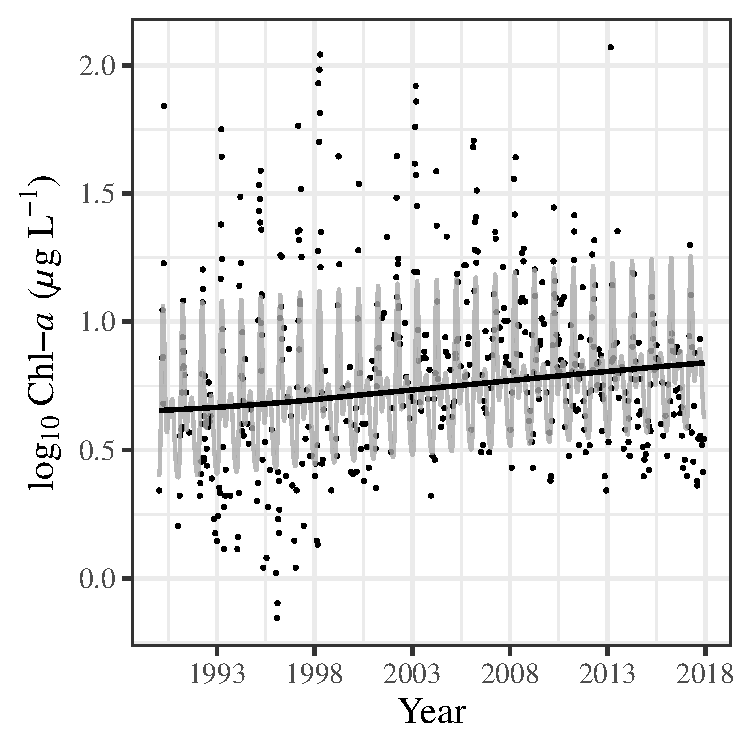
\includegraphics[width = \textwidth, page = 1]{fig/gamex.pdf}
\onslide<2>\includegraphics[width = \textwidth, page = 2]{fig/gamex.pdf}
\onslide<3>\includegraphics[width = \textwidth, page = 3]{fig/gamex.pdf}
\onslide<4>\includegraphics[width = \textwidth, page = 4]{fig/gamex.pdf}
\end{overprint}
\end{figure}
\end{column}
\begin{column}{0.5\textwidth}
\begin{figure}
\begin{overprint}
\onslide<1>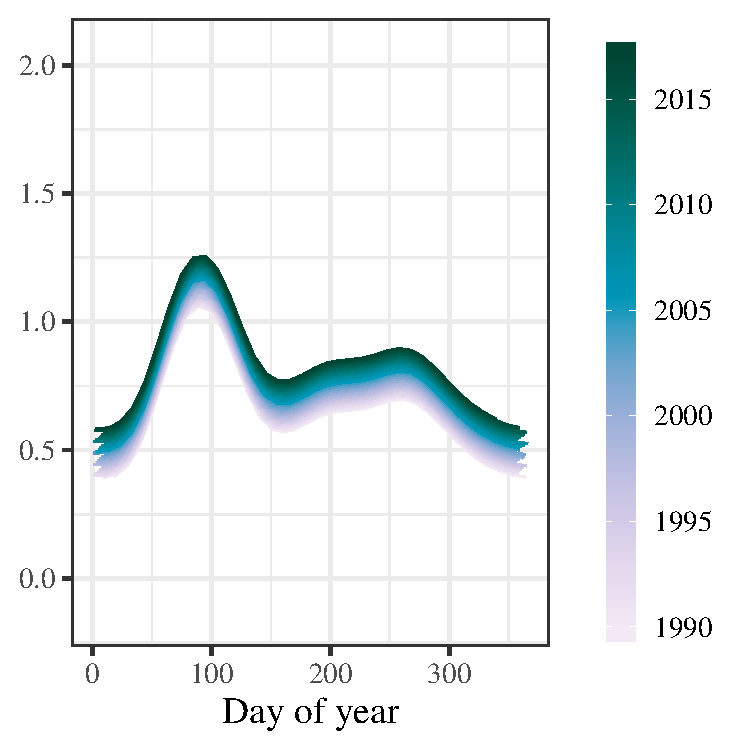
\includegraphics[width = \textwidth, page = 1]{fig/gamex2.pdf}
\onslide<2>\includegraphics[width = \textwidth, page = 2]{fig/gamex2.pdf}
\onslide<3>\includegraphics[width = \textwidth, page = 3]{fig/gamex2.pdf}
\onslide<4>\includegraphics[width = \textwidth, page = 4]{fig/gamex2.pdf}
\end{overprint}
\end{figure}
\end{column}
\end{columns}
\end{frame}

\section{Results}

%%%%%%
\begin{frame}{\textbf{Descriptive results of additive models} \hspace{0pt plus 1 filll} $\vcenter{\hbox{
\includegraphics[width=0.15\paperwidth]{fig/logo.png}}}$}
\vspace{-0.2in}
\begin{center}
\animategraphics[controls,width=\linewidth]{12}{fig/anitst}{}{} %frame rate is 12 per/sec
\end{center}
\end{frame}

%%%%%%
\begin{frame}{\textbf{Descriptive results of additive models} \hspace{0pt plus 1 filll} $\vcenter{\hbox{
\includegraphics[width=0.15\paperwidth]{fig/logo.png}}}$}
Overall comparisons of model structure across stations
\end{frame}

%%%%%%
\begin{frame}{\textbf{Descriptive results of additive models} \hspace{0pt plus 1 filll} $\vcenter{\hbox{
\includegraphics[width=0.15\paperwidth]{fig/logo.png}}}$}
Extension to other response endpoints
\end{frame}

%%%%%%
\begin{frame}{\textbf{Shiny interactive web platform} \hspace{0pt plus 1 filll} $\vcenter{\hbox{
\includegraphics[width=0.15\paperwidth]{fig/logo.png}}}$}
Why do we need this?
Synthesis of results in a communicable format
Answer to specific questions

%%%%%%
Understand implications and limitations of different methods
\end{frame}
\begin{frame}{\textbf{Shiny interactive web platform} \hspace{0pt plus 1 filll} $\vcenter{\hbox{
\includegraphics[width=0.15\paperwidth]{fig/logo.png}}}$}
Example 1
\end{frame}

%%%%%%
\begin{frame}{\textbf{Shiny interactive web platform} \hspace{0pt plus 1 filll} $\vcenter{\hbox{
\includegraphics[width=0.15\paperwidth]{fig/logo.png}}}$}
Example 2
\end{frame}

%%%%%%
\begin{frame}{\textbf{Shiny interactive web platform} \hspace{0pt plus 1 filll} $\vcenter{\hbox{
\includegraphics[width=0.15\paperwidth]{fig/logo.png}}}$}
Example 3
\end{frame}

\section{Conclusions}

%%%%%%
\begin{frame}{\textbf{Summary and next steps} \hspace{0pt plus 1 filll} $\vcenter{\hbox{
\includegraphics[width=0.15\paperwidth]{fig/logo.png}}}$}

\end{frame}


\section{References}

\begin{frame}[t]{\textbf{References}}
\tiny
\setbeamertemplate{bibliography item}{}
\bibliographystyle{apalike_mine}
\bibliography{refs}
\end{frame}

\end{document}
